\documentclass{article}
\usepackage[utf8]{inputenc}
\usepackage[letterpaper,margin=1in]{geometry}
\usepackage{graphicx}
 
\title{\bf{ Lab3: IRQs and Hardware} }

\author{Group 2: Shi Su \& Mengjin Yan}
\date{November 8, 2015}
 
\renewcommand*\contentsname{Content}
 
\begin{document}
 
\maketitle
 
\tableofcontents

\newpage

%%%%%%%%%%%
% OVERVIEW
%%%%%%%%%%%
\section{Overview}
 
On the basis of lab2 to implement a small kernel - {\bf Gravel}, adding the IRQ handling and timer driver.\\
\newline
\begin{figure}[h]
\centering
  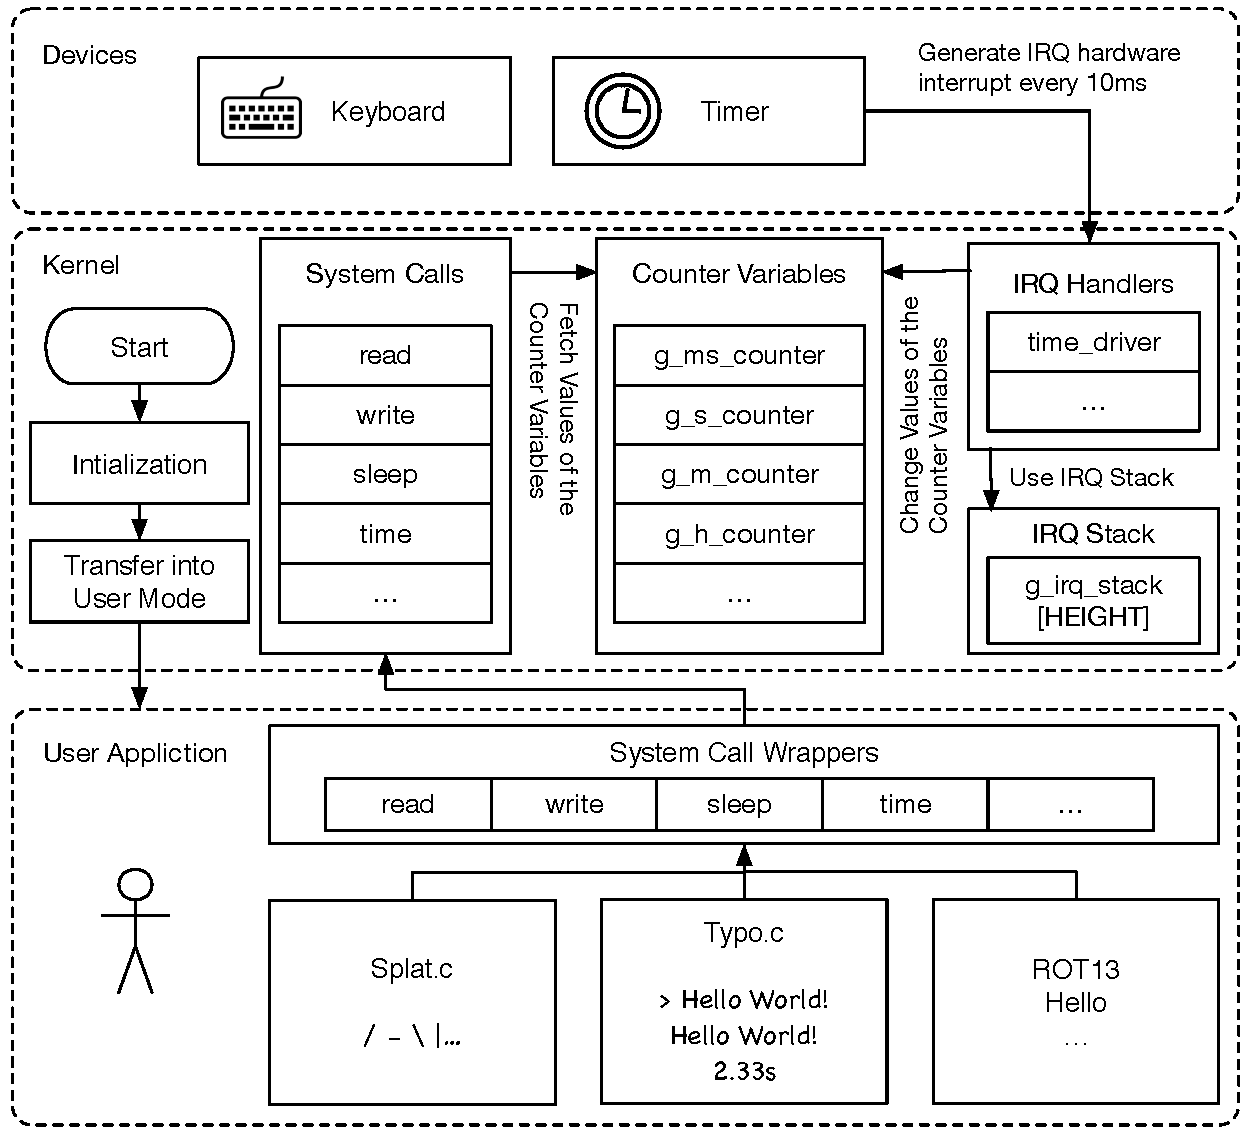
\includegraphics[scale=0.8]{workflow.pdf}\\
 \caption{Modules of Gravel}
 \end{figure}
  
\newpage
\section{Workflow}
\subsection{Kernel Initiation}
\begin{itemize}
	\setlength{\itemsep}{1pt}
	\setlength{\parskip}{0pt}
	\setlength{\parsep}{0pt}
	\item Store the value of r8 (uboot function table) to global variable {\it global\_data}
	\item Wire in SWI/IRQ handler
	\item Set up IRQ stack\\
		A chuck of memory is allocated for IRQ stack in data section as the global variable array {\it g\_irq\_stack}, we don't need to specified its location explicitly and worry about it will be clobbered by code or stack. Since array grows from lower address to higher address, while the growth direction of stack is opposite. So sp is set to point at the highest address(end) of array {\it g\_irq\_stack}. \\
	\item Initiate interrupt controller\\
		Update ICMR to mask interrupt from all interrupt except OSMR0.\\
		Update ICLR to route interrupt from OSMR0 as IRQ.\\
	\item Initiate Timer
		Set all time counter variables to 0.\\
		Set the value of OSSR to 0\\
		Update OIER to enable the interrupt from OSMR0\\
		Set the value of OSMR0 to 32500, which corresponds to 10ms resolution\\
\end{itemize}

%%%%%%%%%%%
% ENTER USER MODE
%%%%%%%%%%%
\subsection{Entering User Mode}
\begin{itemize}
	\setlength{\itemsep}{1pt}
	\setlength{\parskip}{0pt}
	\setlength{\parsep}{0pt}
	\item Store the non-banked register on stack
	\item Store the pointer to supervisor mode stack to global variable {\it g\_svc\_stack}\\
		Follow the same rationale as IRQ stack, we store the pointer to supervisor stack in data section\\
	\item Update cpsr, change mode code to to user mode, unmask IRQ
	\item Set up full descending user mode stack at 0xa3000000
	\item Place the command line arguments from uboot on the user mode stack
	\item Branch to user program loaded at 0xa0000000
\end{itemize}

%%%%%%%%%%%
% IRQ Handing
%%%%%%%%%%%
\subsection{IRQ handling}
When an IRQ interrupt is generated, the system automatically changes into IQR mode and the interrupt is handled by the IRQ handler which is consist of two parts, irq\_handler.S and c\_irq\_handler.c.\\
In irq\_handler.S:
	 \begin{itemize}
	  \setlength{\itemsep}{1pt}
	  \setlength{\parskip}{0pt}
	  \setlength{\parsep}{0pt}
	\item Store non-banked user/supervisor mode register on stack
	\item Branch into c\_swi\_handler
	\end{itemize}
In c\_irq\_handler.c:
	\begin{itemize}
	  \setlength{\itemsep}{1pt}
	  \setlength{\parskip}{0pt}
	  \setlength{\parsep}{0pt}
	\item Read the value of ICMR to determine which device generated the IRQ 
	\item Branch to corresponding ISR
\end{itemize}

%%%%%%%%%%%
% TIMEDRIVER
%%%%%%%%%%%
\subsubsection{Time Driver}	
As shown in the graph, 4 global variables, {\it g\_ms\_counter}, {\it g\_s\_counter}, {\it g\_m\_counter} and {\it g\_h\_counter}, are maintained as time counter in our system. They records how much time has elapsed since kernel booted up. 
 \begin{itemize}
	  \setlength{\itemsep}{1pt}
	  \setlength{\parskip}{0pt}
	  \setlength{\parsep}{0pt}
	  \item {\it g\_ms\_counter} represents the milliseconds
	  \item {\it g\_s\_counter} represents the seconds
	  \item {\it g\_m\_counter} represents the minutes
	  \item {\it g\_h\_counter} represent the hours
\end{itemize}

For every 10ms, an IRQ interrupt is generated from the timer and the system dispatches the interrupt to be handled in the corresponding time\_driver handler. In time\_driver, the corresponding bit in OSSR is cleared and the value of the global variables are updated.\\
\newline
The design of our time counting system successfully separates the register register reading part and the task processing part of the system making it more flexible and convenient when implementing other timer related system calls.
\newline

%%%%%%%%%%%
% SWI Handing
%%%%%%%%%%%
\subsection{SWI handling}
\subsubsection{SWI Handler}
	When user program makes a system call, swi wrapper initiate a swi instruction, which will change the control from user program (user mode) to SWI handler (supervisor mode)\\
\newline
In swi\_handler.S:
	 \begin{itemize}
	  \setlength{\itemsep}{1pt}
	  \setlength{\parskip}{0pt}
	  \setlength{\parsep}{0pt}
	\item Store non-banked user mode register on stack
	\item Restore r8 from global variable {\it global\_data}
	\item Calculate the swi number based on the swi intruction in swi wrapper, put in r0 (arg0)
	\item Put the pointer to the stored registers in r1 (arg1)
	\item With the swi number and register pointer as arguments, branch into c\_swi\_handler
	\end{itemize}
In c\_swi\_handler.c:
	\begin{itemize}
	  \setlength{\itemsep}{1pt}
	  \setlength{\parskip}{0pt}
	  \setlength{\parsep}{0pt}
	\item call the system call functions corresponding to the swi number
	\item put the return value on stack using register pointer, which will be picked up by swi\_handler and passed along through swi wrapper back to user program 
	\end{itemize}
\subsubsection{System Calls}
\begin{itemize}
\item{time}\\
	unsigned long time();\\
	\newline
	{This system call read the value from global time counter: {\it g\_ms\_counter}, {\it g\_s\_counter}, {\it g\_m\_counter}, {\it g\_h\_counter} to calculate the milliseconds that have elapsed since the kernel booted up.}

\item{sleep}\\
	void sleep(unsigned long millis);\\
	\newline
	{This system call reads the start(current) system time using time() system call, and add it with param: millis to get a expected future time before which the program should sleep. Looping until the time() returns a value larger than the expected time.}

\item{read}\\
	ssize\_t read(int fd, void *buf, size\_t count);\\
	\newline
	{Read a requested number of bytes from the given file descriptor, implemented with uboot getc, putc API.}

\item{write}\\
	ssize\_t write(int fd, const void *buf, size\_t count);\\
	\newline
	{Write a requested number of bytes to the given file descriptor, implemented with uboot putc API}

\item{exit}\\
	void exit(int status);\\
	\newline
	{Branch into kernel return flow.}
\end{itemize}

%%%%%%%%%%%
% Test Program
%%%%%%%%%%%
\subsection{Test Programs}
For the test application, we implemented the splat and typo application and make them running correctly on our system. Other applications can be implemented are stop watch and other timer related applications. 
\begin{itemize}
\item{splat}\\
	\newline
	User sleep system call to realize the delay of the state change.\\
	For every 200ms, print out backspace (``/b /b") and the next character in the sequence of ``/ - \ "\\
	Use a while loop to repeat step 2.
\item{typo}\\
	\newline
	After print the prompt, use time system call to get the time for now.\\
	Read the user input and use time system call again to the the end time.\\
	Calculate the time difference and print out the input as well as the time difference.\\
	Use a while loop to repeat step 1~3. 	
\end{itemize}

%%%%%%%%%%%
% EXITING KERNEL
%%%%%%%%%%%
\subsection{Exiting Kernel}
	After return or exit from user mode, the kernel will:
	\begin{itemize}
	  \setlength{\itemsep}{1pt}
	  \setlength{\parskip}{0pt}
	  \setlength{\parsep}{0pt}

	\item Restore supervisor mode stack from global variable {\it g\_svc\_stack}
	\item Restore supervisor mode registers
	\item Restore the native SWI and IRQ handlers
	\item Restore the default value in interrupt controller ICMR and ICLR
	\item Return to gumstix with user program's return value
	\end{itemize}
	
 
\end{document}